\ylDisplay{Päiksekiir kaevupõhjas} % Ülesande nimi
{Tundmatu autor} % Autor
{piirkonnavoor} % Voor
{2000} % Aasta
{P 1} % Ülesande nr.
{1} % Raskustase
{
% Teema: Valgusõpetus
\ifStatement
Sügava kaevupõhja valgustamiseks päikesekiirtega kasutati tasapeeglit, mis oli paigutatud $25^{\circ}$ nurga all vertikaalsuuna suhtes. Kui suure nurga all maapinnast asus Päike?
\fi

\ifHint
Selleks, et valgustada sügava kaevu põhja, peab peeglilt peegeldunud kiir levima vertikaalselt alla.
\fi


\ifSolution
$\alpha = 25^{\circ}$ - nurk peegli ja vertikaalsuuna vahel. Selleks, et valgustada sügava kaevu põhja, peab peeglilt peegeldunud kiir levima vertikaalselt alla.
\begin{center}
	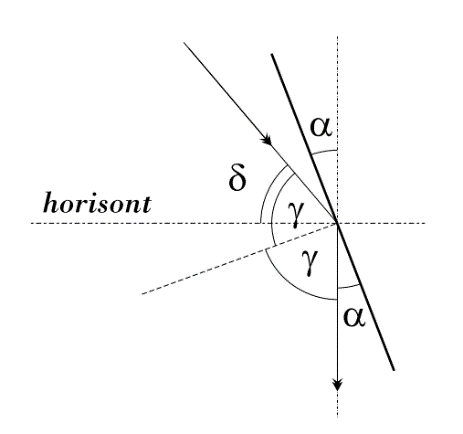
\includegraphics[width=0.5\linewidth]{2000-v2p-01-lah.PNG}
\end{center}
Joonistame kiirte käiku peeglis. Jooniselt leiame, et peegeldusnurk on $\gamma = 90 ^{\circ} - \alpha$
Järelikult Päikese kiire ja horistonaali vaheline nurk on $\delta = 2 \gamma - 90 ^{\circ} = 2 \cdot (90 ^{\circ} - \alpha) - 90 ^{\circ} - 2 \alpha = 40 ^{\circ}$.
\fi
}